\section{Infinite divisibility and a map of processes}\label{ch:sato}

The general theory of infinitely divisible laws is that of two monographs, the standard references for the classes of laws with which this book works: Sato's book on L\'evy processes and infinitely divisible distributions \cite{Sato99} and Bondesson's book on generalised gamma convolutions \cite{Bondesson}. From Sato's book we use the representation of a self decomposable law through its background driving L\'evy process, Yamazato's theorem that self decomposable laws are unimodal, the moment theorem, the uniqueness of the L\'evy Khintchine triplet and, from the later work of Lindner, Pan and Sato \cite{LPS18}, the notion of a quasi infinitely divisible law. From Bondesson's book we use the characterisation of the Laplace transforms of GGCs as hyperbolically completely monotone functions, the behaviour of a GGC at the two ends of its Thorin measure and the closure of the class under weak limits, and from the book of Schilling, Song and Vondra\v{c}ek \cite{boSSV} we take the language of Thorin Bernstein functions.

Five consequences come out (Sections~\ref{sb:sec:sd} to \ref{sb:sec:bernstein}). The centre clock, which is self decomposable with no hypothesis, is driven by a subordinator whose L\'evy density is minus the derivative of the heat trace, and RH is the statement that this density is completely monotone. By Yamazato's theorem the centre clock is unimodal, and so is the shifted clock at every basepoint $\alpha>\frac12$. The law at the basepoint one is subexponential, so that its tail is asymptotic to the tail of its L\'evy measure, which the Thorin density computes. The tilted P\'olya variable $V_\alpha$ is quasi infinitely divisible for every $\alpha>1$ and ceases to be so at $\alpha=1$, where the prime number theorem becomes necessary for its L\'evy form to converge at all. And the subordination identity of Section~\ref{ch:bphit} composes the Laplace exponent of the centre clock, which is known only to be a Bernstein function, with a complete Bernstein function, and the composition is a Thorin Bernstein function for every $\alpha\ge1$; RH is the statement that no composition is needed. None of these results supplies positivity of the Thorin measure uniformly in the height, and Section~\ref{sb:sec:cannot} says why. The laws are also the marginals of processes. Self decomposability makes the centre clock the stationary law of an Ornstein Uhlenbeck process driven by the subordinator above, and the Thorin measure at the basepoint one makes $T_1$ the integral of a gamma process against the inverse of the Poisson smoothed zero count; Section~\ref{ch:riesz} quotes the second, and Section~\ref{pm:sec:wg} derives both and checks them by simulation. Section~\ref{pm:sec:map} adds Brownian motion run on the clocks and places these processes and those of Chapter~\ref{chap:basepoint} on one map, sorted by what each needs: nothing, a zero free half plane, or RH.

We use the notation of Chapter~\ref{chap:basepoint}. The centre clock $T$ has Laplace transform $\varphi_{1/2}(u)=1/G(u)=\xi(\frac12)/\xi(\frac12+\sqrt u)$, and for $\alpha>\frac12$ the shifted clock $T_\alpha$ has Laplace transform $\varphi_\alpha(u)=\xi(\alpha)/\xi(\alpha+\sqrt u)$ and the representation $T_\alpha\stackrel d=\widetilde T_\alpha+H_{\sqrt2(\alpha-\frac12)\widetilde T_\alpha}$ of Theorem~\ref{bp:thm:alpha}, where $\widetilde T_\alpha$ is the centre clock tilted by $e^{-(\alpha-\frac12)^2T}$ and $H_a$ is the first passage time of an independent standard Brownian motion to the level $a$. For $\alpha\ge1$, $T_\alpha$ is a GGC whose Thorin density in the chart $\theta=\sqrt z$ is $v_\alpha/\pi$, with $v_\alpha(\theta)=\re(\xi'/\xi)(\alpha+i\theta)$ (Theorem~\ref{thm:poisson} and \eqref{eq:rho}); at the basepoint one, where the nonvanishing of $\zeta$ on the line $\re s=1$ leaves no zero on that line to contribute an atom, this is the density $\rho_{1/2}=v_1/\pi$ of \eqref{bp:eq:rho1}. We write $b_\alpha=\frac{\xi'}{\xi}(\alpha)$, so that $b_1=\sum_\rho\rho^{-1}=0.0230957089661$, and $V_\alpha$ for the tilted P\'olya variable of Section~\ref{bp:sec:mellin}, the Esscher tilt of the P\'olya density $p$ of \eqref{eq:ch2:mgf} with $\E e^{sV_\alpha}=\xi(\alpha+s)/\xi(\alpha)$, so that $V_{1/2}$ is the P\'olya variable $X$ and $V_1$ is the variable $V$ of Section~\ref{bp:sec:levy}. The scripts are in the folders \texttt{sato\_bondesson} and \texttt{basepoint\_one/process\_map} of the archive, and we name them at each table and figure.

\subsection{Self decomposability: the driving process and unimodality}\label{sb:sec:sd}

The Laplace exponent of the centre clock is $\log G(u)=\int_0^\infty(1-e^{-ut})\,W(t)\,dt/t$, where $W(t)=\sum_ke^{-a_kt}$, with $a_k=-(\rho_k-\frac12)^2$, is the heat trace of the zeros, equal to $\sum_{\gamma>0}e^{-\gamma^2t}$ under RH and to the arithmetic expression \eqref{eq:ch2:Warith} in any case (Section~\ref{ch:clock}). Since $W>0$ and $W'<0$ on $(0,\infty)$ with no hypothesis (Theorem~\ref{thm:ch12:idsd}, whose proof uses the verification of RH below height $1000$), $T$ is infinitely divisible with L\'evy measure $W(t)\,dt/t$, and it is self decomposable. RH holds exactly when $T$ is a GGC, and then its Thorin measure is $\sum_{\gamma>0}\delta_{\gamma^2}$ (Proposition~\ref{prop:rigid}). Self decomposability has a structural consequence that the book has not used so far. A law on $[0,\infty)$ is self decomposable if and only if it is the law of $\int_0^\infty e^{-t}\,dZ_t$ for a subordinator $Z$ with $\E\log(1+Z_1)<\infty$, its background driving L\'evy process \cite{Wolfe82,JurekVervaat83}, \cite[Theorem 17.5]{Sato99}. The L\'evy measure of a self decomposable law on the half line has the form $k(x)\,dx/x$ with $k$ nonincreasing \cite[Corollary 15.11]{Sato99}, and the L\'evy measure of $Z$ then gives mass $k(x)$ to $(x,\infty)$, so that it has the density $-k'(x)$ when $k$ is differentiable. For the centre clock $k=W$, and self decomposability, which is the unconditional statement that $W$ is nonincreasing, gives the following.

\begin{proposition}\label{sb:prop:bdlp}
With no hypothesis, $T\stackrel d=\int_0^\infty e^{-t}\,dZ_t$ for a subordinator $Z$ with L\'evy density $h(x)=-W'(x)$, which is $\sum_{\gamma>0}\gamma^2e^{-\gamma^2x}$ under RH and is given for every $x>0$ by the derivative of the explicit formula \eqref{eq:ch2:Warith} for $W$. The condition $\E\log(1+Z_1)<\infty$ holds because $h$ decays exponentially. Moreover RH holds if and only if $h$ is completely monotone.
\end{proposition}

\begin{proof}
The representation is the theorem of Wolfe and of Jurek and Vervaat applied to the self decomposable law of $T$, and the L\'evy density of $Z$ can be checked directly. If $\Psi_Z(u)=-\log\E e^{-uZ_1}$, the Laplace exponent of $\int_0^\infty e^{-t}\,dZ_t$ is $\int_0^\infty\Psi_Z(ue^{-t})\,dt=\int_0^u\Psi_Z(w)\,dw/w$, so that $\Psi_Z(u)=u(\log G)'(u)$. By Section~\ref{ch:clock}, $(\log G)'(u)=\int_0^\infty e^{-ut}W(t)\,dt$, and since $W(t)=\int_t^\infty h(x)\,dx$ with $h>0$, Fubini's theorem gives
\[
u(\log G)'(u)=\int_0^\infty h(x)\int_0^xue^{-ut}\,dt\,dx=\int_0^\infty\big(1-e^{-ux}\big)h(x)\,dx .
\]
Here $\int_1^\infty h=W(1)$ and $\int_0^1xh(x)\,dx=\int_0^1(W(y)-W(1))\,dy$, which is finite because $W(y)\,dy/y$ is a L\'evy measure, so $h$ is the L\'evy density of a subordinator without drift. It is not integrable at the origin, since $\int_t^1h=W(t)-W(1)$ and $W(t)\sim\log(1/t)/(8\sqrt{\pi t})$ as $t\downarrow0$ (Section~\ref{ch:heat}), so $Z$ makes infinitely many small jumps. As $x\to\infty$, $h(x)\sim\gamma_1^2e^{-\gamma_1^2x}$, which gives $\E\log(1+Z_1)<\infty$ \cite[Theorem 25.3]{Sato99}. For the last statement, $h$ is completely monotone exactly when $W$ is, since $W(x)=\int_x^\infty h$, and complete monotonicity of the heat trace is equivalent to RH (Section~\ref{ch:clock} and Table~\ref{tab:ch3:hierarchy}).
\end{proof}

So the Thorin question for the clock is a question about a single L\'evy process: RH holds exactly when the L\'evy density of the driving process of the centre clock is a mixture of exponentials, and the mixing measure is then $\sum_{\gamma>0}\gamma^2\delta_{\gamma^2}$. Table~\ref{sb:tab:bdlp} checks the arithmetic computation of $h$, obtained by differentiating in $t$ the explicit formula \eqref{eq:ch2:Warith}, that is Weil's formula with the Gaussian test function $e^{-tr^2}$, summed over the primes below $2\times10^4$, against the zero sums over the first $1700$ ordinates. The left panel of Figure~\ref{sb:fig:tail} shows $h$ on $[0.002,0.2]$.

\begin{table}[htbp]
\centering\footnotesize
\setlength{\tabcolsep}{4pt}
\begin{tabular}{rcc}
\toprule
$t$ & $W(t)$, zeros & $W(t)$, explicit formula\\
\midrule
0.005 & 0.537191964091 & 0.537191964091\\
0.01 & 0.149698011254 & 0.149698011254\\
0.02 & 0.0185412917313 & 0.0185412917313\\
0.05 & $4.587835048574\times10^{-5}$ & $4.587835048574\times10^{-5}$\\
0.1 & $2.104799795822\times10^{-9}$ & $2.104799798080\times10^{-9}$\\
\midrule
$t$ & $-W'(t)$, zeros & $-W'(t)$, explicit formula\\
\midrule
0.005 & 165.1022811964 & 165.1022811964\\
0.01 & 33.72924560562 & 33.72924560562\\
0.02 & 3.741068142123 & 3.741068142123\\
0.05 & $9.166117863113\times10^{-3}$ & $9.166117863113\times10^{-3}$\\
0.1 & $4.205189085540\times10^{-7}$ & $4.205189085735\times10^{-7}$\\
\bottomrule
\end{tabular}
\caption{The heat trace $W$ and the L\'evy density $h=-W'$ of the driving process of the centre clock, from the first $1700$ zeros and from the explicit formula \eqref{eq:ch2:Warith} and its derivative with the primes below $2\times10^4$. The explicit columns take the weights $\log p$ in double precision, which accounts for their departure from the zero columns at $t=0.1$. Computed by \texttt{weil.py} in the folder \texttt{sato\_bondesson}.}
\label{sb:tab:bdlp}
\end{table}

The agreement is to all twelve or thirteen digits shown for $t\le0.05$, and at $t=0.1$ to nine digits for $W$ and ten for $h$. At $t=0.1$ the terms of the explicit formula cancel to about nine digits (Table~\ref{tab:ch14:W}), and \texttt{weil.py} takes the weights $\log p$ in double precision; the cancellation magnifies their rounding errors into the differences of $2\times10^{-18}$ in $W$ and $2\times10^{-17}$ in $h$ that the rows at $t=0.1$ show. With the weights in multiple precision and thirty digit arithmetic (\texttt{python3 weil.py mp}) both explicit columns agree with the zero sums at $t=0.1$ to every digit shown, as \eqref{eq:ch2:Warith} does to fifteen digits in Table~\ref{tab:ch2:W}, so the cancellation costs working precision and nothing more. The driving process therefore has the same computational profile as the heat trace: cheap and exact from the primes near the origin, cheap from the zeros away from it.

Yamazato's theorem states that every self decomposable law on the line is unimodal \cite{Yamazato78}, \cite[Theorem 53.1]{Sato99}: its distribution function is convex to the left of some point, a mode, and concave to the right of it. Every GGC is self decomposable (Section~\ref{sec:ch3:hierarchy}), and the centre clock and every shifted clock $T_\alpha$, $\alpha>\frac12$, are self decomposable with no hypothesis (Theorem~\ref{thm:ch12:idsd} and Corollary~\ref{bp:cor:levyalpha}), so we obtain the following.

\begin{corollary}\label{sb:cor:unimodal}
The centre clock is unimodal with no hypothesis, and so is $T_\alpha$ for every $\alpha>\frac12$.
\end{corollary}

Unimodality is a new unconditional property of the centre clock. It does not follow from the Thorin picture, which is conditional at the centre, but from self decomposability, which is not. Self decomposability also goes two steps down the chain of driving processes: the driving process $Z$ of Proposition~\ref{sb:prop:bdlp} and the driving process of $Z$ are self decomposable too, so that their marginals are unimodal with no hypothesis, while the next driving process is not, and the clock lies in Urbanik's class $L_2$ and not in $L_3$ (Theorem~\ref{pk:thm:ladder} and Corollary~\ref{pk:cor:unimodal}). The computed densities (Figure~\ref{sb:fig:unimodal}) have modes near $0.020$ for the centre clock and $0.024$ for $T_1$, and on the computed grids both increase monotonically to the mode and decrease monotonically after it. The grid for the centre clock has spacing $0.0005$, while that for $T_1$ is the geometric grid of the Talbot inversion behind Table~\ref{bp:tab:density}, whose points next to $0.024$ are $0.0175$ and $0.0328$, so the mode of $T_1$ is located only to that accuracy; the value $54.512$ of the density at $0.024$ is the largest on that grid. Yamazato's theorem does not reach the reciprocal zeta law of Section~\ref{ch:rz3}, which is infinitely divisible but not self decomposable (Theorem~\ref{rz:thm:class}), and there the unimodality of the density, which the computations following Proposition~\ref{rz:thm:unimod} support numerically, remains open (Section~\ref{rz:sec:open}).

\begin{figure}[htbp]
\centering
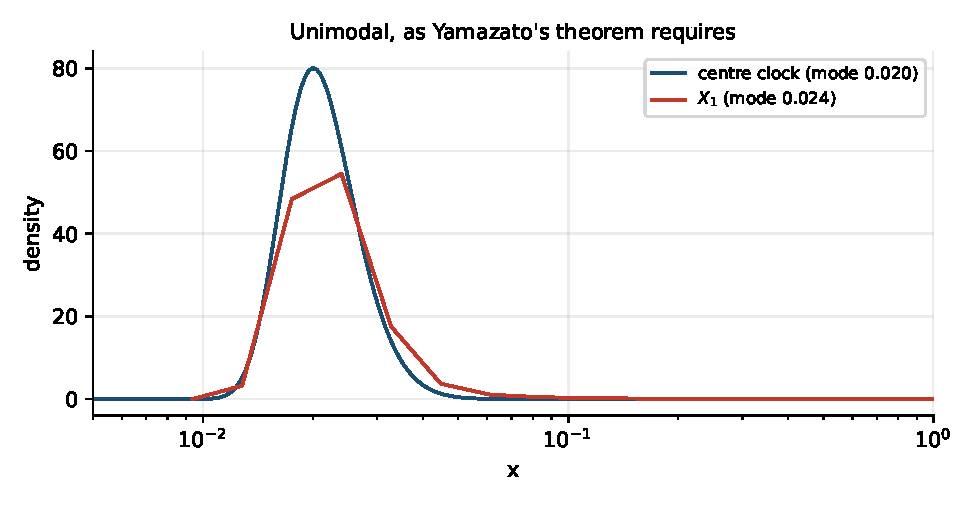
\includegraphics[width=0.75\textwidth]{fig/sb_unimodal.pdf}
\caption{The densities of the centre clock $T$ and of the shifted clock $T_1$, written $X_1$ in the plot, on a logarithmic axis. The density of $T$ is drawn on a grid of spacing $0.0005$ on $[0.004,0.4]$, from the Talbot inversion and the spectral expansion of Section~\ref{ch:clocklaw}; that of $T_1$ on the $40$ point geometric grid of the Talbot inversion behind Table~\ref{bp:tab:density}, which is why its curve is piecewise linear. The legend gives, for each, the grid point of largest density. Assembled by \texttt{comp.py} and drawn by \texttt{figs.py}, both in the folder \texttt{sato\_bondesson}.}
\label{sb:fig:unimodal}
\end{figure}

\subsection{Moments, the tail and the two ends of the Thorin measure}\label{sb:sec:tail}

Sato's moment theorem \cite[Theorem 25.3]{Sato99} says in particular that an infinitely divisible law has finite mean if and only if its L\'evy measure integrates $x$ at infinity. For a GGC with Thorin measure $U$ the L\'evy density is $x^{-1}\int e^{-xz}\,U(dz)$ (Section~\ref{sec:ch3:readings}), so the L\'evy measure $\nu_{T_1}$ of $T_1$ and its tail are, in the chart $\theta=\sqrt z$,
\begin{equation}\label{sb:eq:levy}
\nu_{T_1}(dx)=\frac{dx}x\int_0^\infty e^{-x\theta^2}\rho_{1/2}(\theta)\,d\theta,\qquad \nu_{T_1}((x,\infty))=\int_0^\infty\rho_{1/2}(\theta)\,E_1(x\theta^2)\,d\theta,
\end{equation}
where $E_1(y)=\int_y^\infty e^{-w}\,dw/w$ is the exponential integral. As $x\to\infty$ only $\theta$ near zero contributes, and $\int_0^\infty E_1(w^2)\,dw=\sqrt\pi$ gives $\nu_{T_1}((x,\infty))\sim\rho_{1/2}(0)\sqrt{\pi/x}=b_1(\pi x)^{-1/2}$, which is not integrable at infinity, so the L\'evy measure does not integrate $x$ at infinity and the mean is infinite, as Section~\ref{ch:basepoint} found. The tail is regularly varying of index $-\frac12$, so the L\'evy measure is subexponential. By the theorem of Embrechts, Goldie and Veraverbeke \cite{EGV79}, an infinitely divisible law on $[0,\infty)$ is subexponential if and only if its L\'evy measure, restricted to $(1,\infty)$ and normalised, is subexponential, and if and only if the tail of the law is asymptotic to the tail of the L\'evy measure. Hence
\begin{equation}\label{sb:eq:tail}
P(T_1>x)\sim\nu_{T_1}((x,\infty))\sim\frac{b_1}{\sqrt{\pi x}}=0.01303\,x^{-1/2},\qquad x\to\infty .
\end{equation}
This recovers the tail \eqref{bp:eq:tail}, which Section~\ref{ch:basepoint} found by a Tauberian argument, and the same reasoning, with the Thorin density $v_\alpha/\pi$ and its value $b_\alpha/\pi$ at the origin, gives $\E T_\alpha=\infty$ and the tail $b_\alpha(\pi x)^{-1/2}$ of $T_\alpha$ for every $\alpha\ge1$, and for $\frac12<\alpha<1$ whenever no zero lies to the right of $\alpha$. Theorem~\ref{bp:thm:alpha} gives the infinite mean and the tail of $T_\alpha$ for every $\alpha>\frac12$ by the Tauberian route, and since $T_\alpha$ is infinitely divisible for every $\alpha>\frac12$ (Section~\ref{sb:sec:bernstein}), the theorem of Embrechts, Goldie and Veraverbeke, read from the tail of the law to that of the L\'evy measure, shows that the L\'evy tail of $T_\alpha$ is asymptotic to $b_\alpha(\pi x)^{-1/2}$ as well, wherever the zeros lie.

Table~\ref{sb:tab:tail} and the right panel of Figure~\ref{sb:fig:tail} compare the survival function of $T_1$, computed in Section~\ref{bp:sec:rs1} by Talbot inversion near the origin and by the subordination representation beyond, with the L\'evy tail computed from \eqref{sb:eq:levy} and the Thorin density on $[0,100]$. In the bulk of the law the two differ widely: at $x=0.02$, just below the mode, the survival probability is $0.747$ while the L\'evy tail is $0.101$. Further out the survival probability exceeds the L\'evy tail by $1.2$ per cent at $x=1$, by $0.15$ per cent at $x=10$ and by $0.05$ per cent at $x=100$, and both approach the asymptote of \eqref{sb:eq:tail}; the value $\sqrt{100}\,P(T_1>100)=0.013037$ is the one found in Section~\ref{bp:sec:rs1}.

\begin{table}[htbp]
\centering\small
\begin{tabular}{rcccc}
\toprule
$x$ & $P(T_1>x)$ & $\nu_{T_1}((x,\infty))$ & ratio & $b_1(\pi x)^{-1/2}$\\
\midrule
0.1 & $4.7639\times10^{-2}$ & $4.1558\times10^{-2}$ & 1.1463 & $4.1206\times10^{-2}$\\
0.5 & $1.8907\times10^{-2}$ & $1.8458\times10^{-2}$ & 1.0243 & $1.8428\times10^{-2}$\\
1 & $1.3199\times10^{-2}$ & $1.3041\times10^{-2}$ & 1.0121 & $1.3030\times10^{-2}$\\
10 & $4.1272\times10^{-3}$ & $4.1209\times10^{-3}$ & 1.0015 & $4.1206\times10^{-3}$\\
100 & $1.3037\times10^{-3}$ & $1.3030\times10^{-3}$ & 1.0005 & $1.3030\times10^{-3}$\\
\bottomrule
\end{tabular}
\caption{The subexponential principle for $T_1$: the tail of the law is asymptotic to the tail of its L\'evy measure. The survival function is that of Section~\ref{bp:sec:rs1}, the L\'evy tail is computed from \eqref{sb:eq:levy} with the Thorin density $\rho_{1/2}$ tabulated on $[0,100]$ by \texttt{compute.py} of Section~\ref{ch:basepoint}, the ratio is that of the second column to the third, and the last column is the common asymptote of \eqref{sb:eq:tail}. Computed by \texttt{comp.py} in the folder \texttt{sato\_bondesson}.}
\label{sb:tab:tail}
\end{table}

\begin{figure}[htbp]
\centering
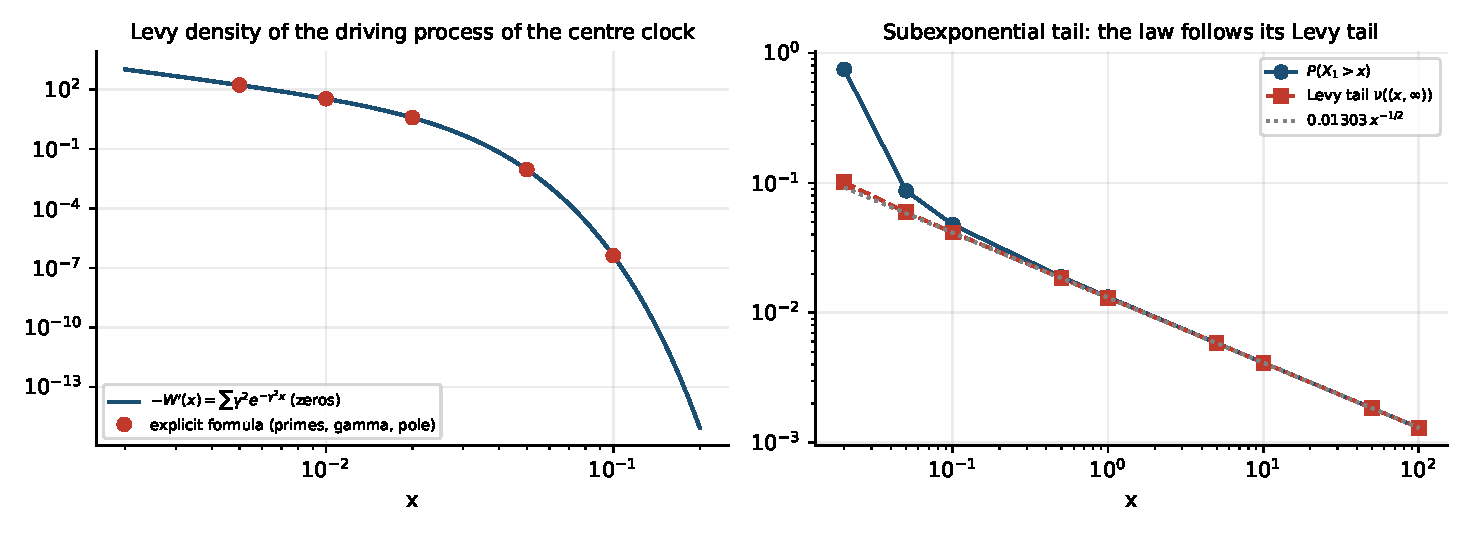
\includegraphics[width=\textwidth]{fig/sb_bdlp_tail.pdf}
\caption{Left: the L\'evy density $h=-W'$ of the driving process of the centre clock on $[0.002,0.2]$, with the heat time $t$ written $x$ in the plot, from the first $1700$ zeros (curve) and from the explicit formula at the five points of Table~\ref{sb:tab:bdlp} (dots). Right: the survival function of $T_1$, written $P(X_1>x)$ in the plot, its L\'evy tail $\nu_{T_1}((x,\infty))$, written $\nu((x,\infty))$, and their common asymptote $b_1(\pi x)^{-1/2}=0.01303\,x^{-1/2}$, at $x=0.02$, $0.05$, $0.1$, $0.5$, $1$, $5$, $10$, $50$ and $100$. Computed by \texttt{weil.py} and \texttt{comp.py} and drawn by \texttt{figs.py}, all in the folder \texttt{sato\_bondesson}.}
\label{sb:fig:tail}
\end{figure}

Bondesson's results on the two ends of the Thorin measure explain the shape of $T_1$: for a GGC the behaviour of the Thorin measure near zero governs the right tail, and its total mass governs the density at the origin \cite{Bondesson}. At the basepoint one the Thorin measure $U_1$ of $T_1$ (Proposition~\ref{bp:prop:thorin}) has $U_1((0,z])=\int_0^{\sqrt z}\rho_{1/2}(\theta)\,d\theta\sim(b_1/\pi)\sqrt z$ as $z\downarrow0$, since $\rho_{1/2}(0)=b_1/\pi$. The substitution $z=uw$ in $-\log\varphi_1(u)=\int\log(1+u/z)\,U_1(dz)$, together with $\int_0^\infty\log(1+1/w)\,d\sqrt w=\pi$, then gives $1-\varphi_1(u)\sim b_1\sqrt u$ as $u\downarrow0$, the Tauberian form of the tail \eqref{sb:eq:tail} and the expansion from which Section~\ref{ch:basepoint} derived \eqref{bp:eq:tail}. At the other end the total mass is infinite, since $U_1((0,Y^2])=M_{1/2}(Y)$ differs from the number $N(Y)$ of zeros with ordinates in $(0,Y]$ by the term $\tau_{1/2}(Y)=O(\log Y)$ of Section~\ref{bp:sec:thorin}, and this is why $T_1$, like the centre clock (Section~\ref{sec:ch19:zones}), is super flat at the origin: its density vanishes faster than any power. Indeed, for every $z_0>0$ the Thorin form gives $\varphi_1(u)\le(1+u/z_0)^{-U_1((0,z_0])}$, and $U_1((0,z_0])\to\infty$ as $z_0\to\infty$, so $\varphi_1(u)$ decays faster than any power of $u$. Markov's inequality $P(T_1\le x)\le e\,\varphi_1(1/x)$ carries this to the distribution function, and since the density $f_{T_1}$ is nondecreasing up to the mode (Corollary~\ref{sb:cor:unimodal}), the bound $xf_{T_1}(x)\le P(T_1\le2x)$ for small $x$ carries it to the density.

\subsection{Uniqueness and quasi infinite divisibility}\label{sb:sec:qid}

The L\'evy Khintchine triplet of an infinitely divisible law is unique \cite[Theorem 8.1]{Sato99}, and when the L\'evy measure has exponential moments it is also determined by the second derivative of the logarithm of the Laplace transform, through the uniqueness of the inverse Laplace transform. Lindner, Pan and Sato \cite{LPS18} call a law quasi infinitely divisible if its characteristic function is the quotient of two infinitely divisible characteristic functions, equivalently if it has a L\'evy Khintchine form with a signed measure $\nu^+-\nu^-$ whose parts $\nu^+$ and $\nu^-$ are both L\'evy measures, so in particular of finite mass away from the origin; the Gaussian coefficient is still nonnegative \cite[Lemma 2.7]{LPS18}, and the triplet is again unique. Their theory places the tilted P\'olya variables $V_\alpha$ precisely. The signed measures in question are those of the L\'evy forms of Section~\ref{bp:sec:levy}: for $\alpha\ge1$,
\[
\log\frac{\xi(\alpha+s)}{\xi(\alpha)}=b_\alpha s+\int_0^\infty\big(e^{-sx}-1+sx\big)\,\Pi_\alpha(dx),
\]
which at $\alpha=1$ is \eqref{bp:eq:levyform}, a compensated limit, and which for $\alpha>1$ converges absolutely when $\re s>1-\alpha$. For $\alpha>1$, read at $s=it$, it is a L\'evy Khintchine form for the characteristic function of $V_\alpha$, with the measure $\Pi_\alpha$ carried to the negative half line by the reflection $x\mapsto-x$. We write $x_*=0.28120$ for the root of $e^{-3x}=1-e^{-2x}$, which is the logarithm of the real root $1.32472$ of $y^3=y+1$, the plastic number.

\begin{proposition}\label{sb:prop:qid}
\begin{enumerate}
\item The P\'olya variable $X=V_{1/2}$ is not quasi infinitely divisible, since its characteristic function $\Xi(t)/\Xi(0)$ vanishes at the ordinates.
\item For every $\alpha>1$, $V_\alpha$ is quasi infinitely divisible and not infinitely divisible. Its signed L\'evy measure is the reflection to the negative half line of
\[
\Pi_\alpha(dx)=\Big(\frac{e^{-(\alpha+2)x}}{1-e^{-2x}}-e^{-(\alpha-1)x}\Big)\frac{dx}x+\sum_n\frac{\Lambda(n)}{n^\alpha\log n}\,\delta_{\log n}(dx),
\]
whose atoms have total mass $\log\zeta(\alpha)$ and whose absolutely continuous part is positive on $(0,x_*)$ and negative beyond. The negative part of $\Pi_\alpha$ is therefore carried by $(x_*,\infty)$, and its mass on $(1,\infty)$ is $E_1(\alpha-1)-\sum_{k\ge0}E_1(\alpha+2+2k)$: it is dominated by the pole term $e^{-(\alpha-1)x}dx/x$, of mass $E_1(\alpha-1)$ on $(1,\infty)$, but is not equal to it.
\item At $\alpha=1$, $V_1$ is not quasi infinitely divisible. The candidate measure $\Pi_1$ of Proposition~\ref{bp:prop:levy} has the pole term $-dx/x$ and the prime atoms $\Lambda(n)/(n\log n)$ at $\log n$, each of infinite mass on $(1,\infty)$; since the gamma density $e^{-3x}(1-e^{-2x})^{-1}/x$ is less than $0.06/x$ there, the positive and the negative part of $\Pi_1$ both have infinite mass on $(1,\infty)$, and its L\'evy form converges only as a compensated limit, which exists by the prime number theorem.
\end{enumerate}
\end{proposition}

Items (1) and (2) are due to Nakamura \cite{Nakamura15}: (2), with the same measure, is his Theorem 1.4, and (1) is the remark after it.

\begin{proof}
(1) A quasi infinitely divisible characteristic function is the exponential of the finite exponent of its L\'evy Khintchine form, so it never vanishes, while $\E e^{itX}=\Xi(t)/\Xi(0)$ by \eqref{eq:ch2:mgf}, which vanishes at $t=14.134725$ and at every other ordinate of a zero on the critical line.

(2) Let $\alpha>1$. Every piece of the L\'evy form then converges absolutely, and each piece is a L\'evy measure: the positive density $e^{-(\alpha+2)x}(1-e^{-2x})^{-1}dx/x$, the pole term and the atoms. The factorisation of $\xi$ exhibits the two infinitely divisible laws of the definition. Removing the factor $s(s-1)$ from $\xi(s)=\frac12s(s-1)\pi^{-s/2}\Gamma(\frac s2)\zeta(s)$ gives, for $\re s>1-\alpha$,
\[
\frac{\xi(\alpha+s)}{\xi(\alpha)}\cdot\frac{\alpha}{\alpha+s}\cdot\frac{\alpha-1}{\alpha-1+s}=\pi^{-s/2}\,\frac{\Gamma(\frac{\alpha+s}2)}{\Gamma(\frac\alpha2)}\,\frac{\zeta(\alpha+s)}{\zeta(\alpha)} .
\]
Let $e_1$ and $e_2$ be standard exponential variables, $\Gamma_{\alpha/2}$ a gamma variable of shape $\frac\alpha2$ and unit scale, and $\mathcal Z_\alpha$ a variable with the zeta law $P(\mathcal Z_\alpha=n)=n^{-\alpha}/\zeta(\alpha)$, all independent of each other and of $V_\alpha$. Since $\E e^{-se_1/\alpha}=\alpha/(\alpha+s)$, $\E\Gamma_{\alpha/2}^{s/2}=\Gamma(\frac{\alpha+s}2)/\Gamma(\frac\alpha2)$ and $\E\mathcal Z_\alpha^{-s}=\zeta(\alpha+s)/\zeta(\alpha)$, the identity says that
\[
V_\alpha-\frac{e_1}\alpha-\frac{e_2}{\alpha-1}\stackrel d=\frac12\log\Gamma_{\alpha/2}-\frac12\log\pi-\log\mathcal Z_\alpha .
\]
The right side is infinitely divisible: $\frac12\log\Gamma_{\alpha/2}$ has, by Binet's formula \cite[\S5.9]{DLMF} as in the proof of Proposition~\ref{bp:prop:levy}, the L\'evy measure $e^{-\alpha x}(1-e^{-2x})^{-1}dx/x$ reflected to the negative half line, and by the Euler product $-\log\mathcal Z_\alpha$ is compound Poisson with L\'evy measure $\sum_n\Lambda(n)(n^\alpha\log n)^{-1}\delta_{-\log n}$, of total mass $\log\zeta(\alpha)$. The variable $-e_1/\alpha-e_2/(\alpha-1)$ is infinitely divisible as well, with L\'evy measure $(e^{-\alpha x}+e^{-(\alpha-1)x})\,dx/x$ reflected, so the law of $V_\alpha$ convolved with an infinitely divisible law is infinitely divisible, and $V_\alpha$ is quasi infinitely divisible. Its signed L\'evy measure is the difference of the two L\'evy measures, which is $\Pi_\alpha$ reflected, since $e^{-\alpha x}(1-e^{-2x})^{-1}-e^{-\alpha x}=e^{-(\alpha+2)x}(1-e^{-2x})^{-1}$. The absolutely continuous part of $\Pi_\alpha$ has the density $e^{-(\alpha-1)x}\big(e^{-3x}(1-e^{-2x})^{-1}-1\big)x^{-1}$, whose sign is that of $e^{-3x}-(1-e^{-2x})$ whatever $\alpha$ is: positive on $(0,x_*)$ and negative beyond, where it is at least $-e^{-(\alpha-1)x}/x$, whose integral over $(1,\infty)$ is $E_1(\alpha-1)$; expanding $(1-e^{-2x})^{-1}$ in powers of $e^{-2x}$ and integrating termwise over $(1,\infty)$ gives the mass of the negative part there. If $V_\alpha$ were infinitely divisible, uniqueness of the triplet \cite[Theorem 8.1]{Sato99}, applied to the identity in law above, would make its L\'evy measure equal to $\Pi_\alpha$ reflected, which is negative on the reflection of $(x_*,\log2)$, an interval that carries no atom. So $V_\alpha$ is not infinitely divisible.

(3) Suppose that $V_1$ is quasi infinitely divisible, so that $\E e^{itV_1}=\exp\Psi_{V_1}(t)$ with
\[
\Psi_{V_1}(t)=ict-\frac A2t^2+\int_{\R}\big(e^{ity}-1-ity\mathbf 1\{|y|\le1\}\big)\,\mu(dy),
\]
where $A$ and $c$ are real and $\mu$ is a signed measure on $\R\setminus\{0\}$ with $\int\min(1,y^2)\,|\mu|(dy)<\infty$. As in (1), the characteristic function never vanishes, so $\xi(1+it)\ne0$ for real $t$; and $\xi(1+s)\ne0$ for $\re s>0$ by the Euler product. So $\ell(s)=\log(\xi(1+s)/\xi(1))$, with $\ell(0)=0$, is a continuous logarithm on the closed half plane $\re s\ge0$, holomorphic inside, and $\Psi_{V_1}(t)=\ell(it)$, since both are continuous logarithms of $\xi(1+it)/\xi(1)$ that vanish at $t=0$. For $r>0$ put $\Delta_rF(t)=F(t+r)+F(t-r)-2F(t)$. Then
\[
\Delta_r\Psi_{V_1}(t)=\int_{\R}e^{ity}\,\lambda_r(dy),\qquad \lambda_r(dy)=-Ar^2\delta_0(dy)+(2\cos ry-2)\,\mu(dy),
\]
and $\lambda_r$ is a finite signed measure because $|2\cos ry-2|\le\min(4,r^2y^2)$. On the other side, let $\check\Pi_1$ be the reflection of $\Pi_1$ to the negative half line. For $\sigma>0$ the variable $V_{1+\sigma}$ has the characteristic function $\exp(\ell(\sigma+it)-\ell(\sigma))$, and by (2) its signed L\'evy measure is the reflection of $\Pi_{1+\sigma}(dx)=e^{-\sigma x}\Pi_1(dx)$, that is $e^{\sigma y}\check\Pi_1(dy)$. The second difference removes the drift and the compensator, so
\[
\Delta_r\ell(\sigma+i\,\cdot\,)(t)=\int_{\R}e^{ity}\,m_\sigma(dy),\qquad m_\sigma(dy)=e^{\sigma y}(2\cos ry-2)\,\check\Pi_1(dy),
\]
where $m_\sigma$ is a finite signed measure, the atoms contributing at most $4\log\zeta(1+\sigma)$ to its total variation. As $\sigma\downarrow0$, $m_\sigma$ tends to $m_0=(2\cos ry-2)\,\check\Pi_1$ in the space of tempered distributions, by dominated convergence, because $|m_0|$ is locally finite and $|m_0|((-R,0))=O(R)$ as $R\to\infty$: the factor $2\cos ry-2$ tames $\check\Pi_1$ near the origin, and $\Lambda(n)\le\log n$ bounds the atom at $-\log n$ by $1/n$. So the Fourier transforms converge as tempered distributions. On the other hand $\Delta_r\ell(\sigma+it)\to\Delta_r\Psi_{V_1}(t)$ uniformly for $t$ in compact sets, because $\ell$ is uniformly continuous on compact subsets of the closed half plane. Hence the Fourier transforms of $m_0$ and $\lambda_r$ agree on smooth test functions of compact support, which are dense in the Schwartz space, so they agree as tempered distributions, and since the Fourier transform is injective there, $m_0=\lambda_r$ as measures. The mass at the origin gives $A=0$. On a compact set $K\subset\R\setminus\{0\}$, $2\cos ry-2<0$ once $r<2\pi/\max_K|y|$, so $\mu=\check\Pi_1$ on $K$, and hence on $\R\setminus\{0\}$. But the atom of $\Pi_1$ at $\log p$ has mass $1/p$, so $|\mu|((-\infty,-1))\ge\sum_{p\ge3}1/p=\infty$, and $|\mu|$ is not a L\'evy measure. This contradiction proves (3).
\end{proof}

In the identity in law used for (2) the two infinitely divisible witnesses fail together at $\alpha=1$: the exponential variable $e_2/(\alpha-1)$, which carries the pole of $\zeta$, and the zeta law of $\mathcal Z_\alpha$, which carries the primes, both cease to exist. So quasi infinite divisibility is lost exactly at the basepoint one, the same place where the prime number theorem becomes necessary and where the L\'evy form turns from absolutely to conditionally convergent.

The proof of (3) uses about the primes only the Euler product, and not the prime number theorem: the nonvanishing of $\zeta$ on the line $\re s=1$, the first step towards that theorem, enters only through the hypothesis, which forces it. The existence of the compensated limit in (3) needs more. Of the two estimates that the proof of Proposition~\ref{bp:prop:levy} uses for it, the second is the logarithm of Mertens' product theorem \cite[Theorem 429]{boHardyWright} and gives the cancellation of zeroth order between the prime atoms and $dx/x$, while the first, which the compensator $sx$ requires, is a form of the prime number theorem, whose analytic proof rests on $\zeta(1+it)\ne0$ \cite{Titchmarsh}. Below the basepoint one the L\'evy form exists only if there is a zero free half plane (Proposition~\ref{bp:prop:below}).

Section~\ref{bp:sec:levy} reads the conclusion of (3) from the L\'evy form itself, and the proof of (3) supplies the uniqueness on which that reading rests, namely that no other signed measure can represent the same characteristic function. Since an infinitely divisible law is quasi infinitely divisible, (3) also shows directly that $V_1$ is not infinitely divisible, which is how that section concludes. The same argument, with $\xi(1+s,\chi_{12})$ in place of $\xi(1+s)$, shows that the tilted eta variable of Section~\ref{bp:eta:sec:levy} is neither quasi infinitely divisible nor infinitely divisible, as that section argues: its L\'evy form has the atoms $\chi_{12}(n)\Lambda(n)/(n\log n)$ at $\log n$, of absolute value $1/p$ at $\log p$ for every prime $p\ge5$, and by Dirichlet's theorem those with $\chi_{12}(n)=1$ and those with $\chi_{12}(n)=-1$ both have infinite mass.

\subsection{Bondesson's classes and Thorin Bernstein functions}\label{sb:sec:bernstein}

By Bondesson's characterisation, recalled in Section~\ref{sec:ch3:hierarchy}, a function with limit one at the origin is the Laplace transform of a GGC if and only if it is hyperbolically completely monotone \cite[Theorem 6.1.1]{Bondesson}, and the class of HCM densities is closed under products and quotients of independent variables and under powers $X^q$ with $|q|\ge1$ \cite[Section 5.1]{Bondesson}. These are the tools behind the Bosch threshold of Theorem~\ref{bs:thm:power}: $\varphi_{1/2}(u^{1/\beta})$ is HCM exactly when $|\beta|\ge1/(1-\alpha_\xi)$, where $\alpha_\xi=2\delta_*/\pi$ and $\delta_*$ is the largest angle $|\arg\gamma|$ over the zeros $\gamma$ of $\Xi$ with $\re\gamma>0$. RH is the statement $\alpha_\xi=0$.

The class of GGCs is closed under weak limits (Section~\ref{sec:weak:limits}), which gives the closure criterion of Corollary~\ref{cor:weak:closure} used for the Kent approximants of Section~\ref{sec:ch18:kent}. Bondesson also treats mixtures of exponential laws and their generalised convolutions. This is the natural class for Kent's hitting times started from an interior point: for a diffusion started at $x_0$ and a level $y_0>x_0$ the Laplace transform of the first passage time to $y_0$ is $\psi_u(x_0)/\psi_u(y_0)$, where $\psi_u$ is the increasing positive solution of $\mathcal A\psi=u\psi$ for the generator $\mathcal A$ of the diffusion, and it is a ratio of two products with interlacing zeros. The law of $T_1$ is not a mixture of exponentials, since a mixture of exponentials has a completely monotone density while that of $T_1$ vanishes at the origin and has an interior mode (Figure~\ref{sb:fig:unimodal}). This is consistent with the conclusion of Section~\ref{ch:bphit} that $T_1$ is a subordinated rather than a direct Kent hitting time (Section~\ref{bp:sec:kent} and Theorem~\ref{bp:thm:sub}).

In the language of Schilling, Song and Vondra\v{c}ek \cite[Definition 9.10]{boSSV}, a law on $[0,\infty)$ is a GGC exactly when its Laplace exponent is a Thorin Bernstein function, equivalently when the derivative of the exponent is a Stieltjes function, the function $f_H$ of Section~\ref{sec:ch3:readings}. The Laplace exponent of the centre clock is $\log G$, a Bernstein function with no hypothesis because $T$ is infinitely divisible; we give it no separate name, since $G$ already denotes the reciprocal of its Laplace transform. The subordination identity of Theorem~\ref{bp:thm:alpha} reads
\begin{equation}\label{sb:eq:comp}
\begin{gathered}
-\log\varphi_\alpha(u)=\log G\big((\alpha-\tfrac12)^2+f_\alpha(u)\big)-\log G\big((\alpha-\tfrac12)^2\big),\\
f_\alpha(u)=u+2(\alpha-\tfrac12)\sqrt u,
\end{gathered}
\end{equation}
with $f_\alpha$, the Laplace exponent of the subordinator $\sigma^{(\alpha)}$ of that theorem, a complete Bernstein function. The derivative $\frac{d}{du}[-\log\varphi_\alpha(u)]=\frac1{2\sqrt u}\frac{\xi'}{\xi}(\alpha+\sqrt u)$ is a Stieltjes function exactly when no zero lies to the right of $\alpha$, that is when $\alpha\ge\sup_\rho\re\rho$, which is the criterion of Theorem~\ref{thm:poisson}: a zero with $\re\rho>\alpha$ makes $\xi(\alpha+\sqrt u)$ vanish at the point $u=(\rho-\alpha)^2$ of the cut plane $\cut$, where a Stieltjes function is holomorphic. This is a statement about the analytic continuation of the exponent, and not about the sign of the Thorin density $v_\alpha/\pi$ on the single line $\re s=\alpha$, which is not known to exclude zeros to the right of that line (Remark~\ref{rem:ch2:oneline}).

\begin{proposition}\label{sb:prop:tbf}
For every $\alpha\ge1$ the composition $\log G((\alpha-\frac12)^2+f_\alpha)-\log G((\alpha-\frac12)^2)$ is a Thorin Bernstein function with no hypothesis, while $\log G$ itself is a Thorin Bernstein function if and only if RH holds. For $\frac12<\alpha<1$ the composition is a Thorin Bernstein function if and only if $\zeta$ has no zeros with real part greater than $\alpha$.
\end{proposition}

\begin{proof}
By \eqref{sb:eq:comp} the composition is the Laplace exponent of $T_\alpha$, so it is a Thorin Bernstein function exactly when $T_\alpha$ is a GGC, which by Theorem~\ref{thm:poisson} happens exactly when no zero has real part greater than $\alpha$. For $\alpha\ge1$ there is none, since $\zeta$ has no zeros on or to the right of the line $\re s=1$. The exponent $\log G$ is a Thorin Bernstein function exactly when $T$ is a GGC, which is RH by Proposition~\ref{prop:rigid}.
\end{proof}

For every $\alpha>\frac12$ the composition is at least a Bernstein function: $u\mapsto\log G((\alpha-\frac12)^2+u)-\log G((\alpha-\frac12)^2)$ is the Laplace exponent of the tilted clock $\widetilde T_\alpha$, and a Bernstein function composed with a Bernstein function is again one \cite[Corollary 3.8]{boSSV}. So $T_\alpha$ is infinitely divisible for every $\alpha>\frac12$ with no hypothesis, and the location of the zeros decides only whether it is a GGC. The proposition says that composing with the complete Bernstein function $f_\alpha$ creates the Thorin property from a function only known to be Bernstein. Analytically this is the Poisson smoothing of the Thorin measure by Cauchy kernels of widths $\alpha-\beta$ (Proposition~\ref{prop:struct}); probabilistically it is the stable one half subordination of Theorem~\ref{bp:thm:alpha}, by a drift plus a stable subordinator of index one half. RH is the statement that the smoothing was never needed, that is, that $\log G$ is already a Thorin Bernstein function, and the family $\alpha\downarrow\frac12$ measures how much smoothing is required at each basepoint.

General composition theorems do not settle this. For a Bernstein function $\kappa$ and $a\ge0$ let $\kappa_a(u)=\kappa((\sqrt u+a)^2)-\kappa(a^2)$, so that the composition in \eqref{sb:eq:comp} is $\kappa_a$ for $\kappa=\log G$ and $a=\alpha-\frac12$. If $\kappa$ is a Thorin Bernstein function then so is every $\kappa_a$, because the shift turns a drift $cu$ into $c(u+2a\sqrt u)$ and each factor $(1+u/t)^{-1}$ of the Thorin form into $(a^2+t)/((\sqrt u+a)^2+t)$, the Laplace transform of a GGC whose Thorin density in $\theta$ is the pair of Cauchy kernels of width $a$ at $\pm\sqrt t$, as in Section~\ref{bp:sec:sub}. Applied to $\kappa_a$, with $\kappa_{a+a'}=(\kappa_a)_{a'}$, this shows that the shifts $a$ for which $\kappa_a$ is a Thorin Bernstein function form a half line, and for $\kappa=\log G$ Proposition~\ref{sb:prop:tbf} identifies it as $[a_*,\infty)$ with $a_*=\sup_\rho\re\rho-\frac12$; RH is the statement $a_*=0$. For a fixed shift the implication cannot be reversed. The function $\kappa(u)=2\log(1+u)+\log(1+(120u+16u^2)/289)$ is a Bernstein function, since $\kappa'$ is the Laplace transform of $2e^{-x}+2e^{-15x/4}\cos2x\ge0$, and it is not a Thorin Bernstein function, since $\kappa'$ has poles at $-\frac{15}4\pm2i$, where a Stieltjes function is holomorphic; yet
\[
\kappa_{1/2}(u)=\log\Big(1+\frac u4\Big)+2\log\frac{4((\sqrt u+\frac12)^2+1)}5+\log\frac{(\sqrt u+1)^2+4}5
\]
is a Thorin Bernstein function, the exponent of an exponential law plus the exponents of GGCs whose Thorin densities are pairs of Cauchy kernels, of width $\frac12$ at $\pm1$ and of width $1$ at $\pm2$; the function $u\mapsto\kappa(u/4a^2)$ gives the same example at any shift $a>0$.

The Dirichlet mean representation of James, Roynette and Yor \cite{JRY} writes a GGC whose Thorin measure has finite total mass $c$ as the product $\Gamma_c\mathcal M$ of a gamma variable $\Gamma_c$ of shape $c$ and an independent Dirichlet mean $\mathcal M$. It applies to the truncated lattice variables $\mathcal S_n$ of Section~\ref{rz:sec:finite}, whose Thorin measures have total mass $2n$, and to the finite sums of exponential variables of Proposition~\ref{rz:prop:multlee}, but not to $T_\alpha$ or, under RH, to $T$, whose Thorin measures have infinite mass.

\subsection{What these results cannot give}\label{sb:sec:cannot}

Every GGC criterion in these books is, for the reciprocal Xi function at the centre, equivalent to RH: the HCM property of the Laplace transform and the Stieltjes property of the derivative of the exponent (Theorem~\ref{bh:thm:main}), the Pick function property (Corollary~\ref{bs:cor:rh}), and the complete monotonicity of the L\'evy density of the driving process (Proposition~\ref{sb:prop:bdlp}). The books classify laws and derive consequences once positivity of the Thorin measure is known, and the consequences obtained in Sections~\ref{sb:sec:sd} to \ref{sb:sec:bernstein}, the driving process, unimodality, the subexponential tail, quasi infinite divisibility and the Thorin Bernstein compositions, are mostly unconditional. Table~\ref{sb:tab:results} collects them with their sources.

They are unconditional for one of two reasons. Some use only the infinite divisibility and self decomposability of the centre clock, that is the inequalities $W>0$ and $W'<0$, which hold wherever the zeros above height $1000$ lie, their proof using only the verification of RH below that height (Theorem~\ref{thm:ch12:idsd}). The others use the region $\re s\ge1$, through positivity of the Thorin measure at a basepoint $\alpha\ge1$, which rests on the nonvanishing of $\zeta$ on the line $\re s=1$ (Theorem~\ref{thm:poisson}), or through the Euler product, as in Proposition~\ref{sb:prop:qid}. Neither source reaches below the basepoint one: the first cannot detect the higher zeros at all, and the second stops at the line $\re s=1$, where the Euler product ceases to converge. So none of the results supplies positivity of the Thorin measure uniformly in the height at a basepoint $\alpha<1$, in the sense of Theorem~\ref{thm:poisson} that $T_\alpha$ is a GGC, which is the zero free half plane $\re s>\alpha$ of step~7 of the path in Table~\ref{tab:ch25:path}, and still less at the centre, where it is RH itself. That positivity, uniform in the height, is the one ingredient still missing on the path to RH; the half plane $\re s>\frac78$ announced in October 2026 would supply it for every $\alpha>\frac78$, by arithmetic from outside the theory (Section~\ref{sec:ch25:open}).

\begin{table}[htbp]
\centering\small
\begin{tabular}{p{0.24\textwidth}p{0.2\textwidth}p{0.35\textwidth}p{0.09\textwidth}}
\toprule
result & source & consequence here & status\tabularnewline
\midrule
\raggedright background driving L\'evy process & \raggedright Wolfe; Jurek and Vervaat; Sato, Theorem 17.5 & \raggedright centre clock driven by a subordinator with L\'evy density $-W'$; RH if and only if it is completely monotone & proved\tabularnewline
\raggedright Yamazato's theorem & \raggedright Yamazato; Sato, Theorem 53.1 & \raggedright centre clock and $T_\alpha$, $\alpha>\frac12$, unimodal & proved\tabularnewline
\raggedright Urbanik's classes $L_n$ & \raggedright Urbanik; Sato 1980; Berg and Forst & \raggedright centre clock in $L_2$, not in $L_3$; its driving process and the driving process of that self decomposable, with unimodal marginals & proved\tabularnewline
\raggedright moment theorem & \raggedright Sato, Theorem 25.3 & \raggedright $\E T_\alpha=\infty$ for $\alpha\ge1$ & proved\tabularnewline
\raggedright subexponential tails & \raggedright Embrechts, Goldie, Veraverbeke & \raggedright $P(T_\alpha>x)\sim b_\alpha(\pi x)^{-1/2}$; ratio $1.0005$ at $x=100$ & \raggedright proved, checked\tabularnewline
\raggedright uniqueness, quasi infinite divisibility & \raggedright Sato, Theorem 8.1; Lindner, Pan, Sato & \raggedright $V_\alpha$ quasi infinitely divisible for $\alpha>1$, not at $\alpha=1$; P\'olya variable not quasi infinitely divisible & proved\tabularnewline
\raggedright HCM characterisation and closure & \raggedright Bondesson & \raggedright Bosch threshold for powers & proved\tabularnewline
\raggedright Thorin measure at the two ends & \raggedright Bondesson & \raggedright $x^{-1/2}$ tail and super flat origin & proved\tabularnewline
\raggedright Thorin Bernstein composition & \raggedright Schilling, Song, Vondra\v{c}ek & \raggedright smoothing by $f_\alpha$ creates the Thorin property for $\alpha\ge1$ & proved\tabularnewline
\raggedright Dirichlet means & \raggedright James, Roynette, Yor & \raggedright applies to truncations only & remark\tabularnewline
\bottomrule
\end{tabular}
\caption{What the books of Sato and Bondesson, and the papers around them, give the reciprocal Xi function: each result used in this section, its source, its consequence for the centre clock $T$, the shifted clocks $T_\alpha$ and the tilted P\'olya variables $V_\alpha$, and its status. Theorem numbers, here and in the text, refer to the first edition of Sato's book \cite{Sato99}.}
\label{sb:tab:results}
\end{table}

What the two books do provide is a vocabulary in which RH can be stated in several equivalent forms, each with its own tools: a subordinator whose L\'evy density must be shown to be a mixture of exponentials, a Bernstein function whose derivative must be shown to be a Stieltjes function, and a smoothing by $f_\alpha$ that must be shown to be unnecessary. Section~\ref{ch:path} collects the steps of the Thorin approach, marks each as proved, computed, announced or open, and sets out the path along which positivity would have to be carried from the basepoint one to the centre. The same laws are the marginals of stochastic processes, and Sections~\ref{pm:sec:wg} and \ref{pm:sec:map} collect these processes, with those of Sections~\ref{ch:bphit} and \ref{ch:strip}, on one map.

\subsection{Wiener gamma integrals and the Riemann Ornstein Uhlenbeck process}\label{pm:sec:wg}

A GGC is a superposition of gamma laws, and a gamma process realises the superposition pathwise. Let $(\Gamma_t)_{t\ge0}$ be a standard gamma process, the subordinator with $\E e^{-u\Gamma_t}=(1+u)^{-t}$, so that $\Gamma_t$ has the gamma law of shape $t$ and unit scale, like the variables $\Gamma_{\alpha/2}$ and $\Gamma_c$ of Sections~\ref{sb:sec:qid} and \ref{sb:sec:bernstein}. For a measurable $f\ge0$ the Wiener integral $\int_0^\infty f(t)\,d\Gamma_t$ has Laplace exponent $\int_0^\infty\log(1+uf(t))\,dt$. Let $U$ be the Thorin measure of a GGC without drift, $M(\theta)=U((0,\theta^2])$ its cumulative mass in the chart $\theta=\sqrt z$, and $M^{-1}(t)=\inf\{\theta:M(\theta)>t\}$ the right continuous inverse. The image of Lebesgue measure on $(0,M(\infty))$ under $M^{-1}$ is $dM$, so the substitution $t=M(\theta)$ turns $\int_0^\infty\log(1+u/M^{-1}(t)^2)\,dt$ into $\int\log(1+u/z)\,U(dz)$, and the GGC is the Wiener gamma integral
\begin{equation}\label{pm:eq:wg}
\int_0^\infty\frac{d\Gamma_t}{M^{-1}(t)^2},
\end{equation}
which is the Wiener gamma representation of the class \cite{JRY}. At the centre, under RH, $M$ is the zero counting function $N$, $M^{-1}(t)=\gamma_k$ for $k-1\le t<k$, the ordinates being counted in increasing order and with multiplicity, and \eqref{pm:eq:wg} is $\sum_k(\Gamma_k-\Gamma_{k-1})/\gamma_k^2$, the series $\sum_{\gamma>0}e_\gamma/\gamma^2$ of Proposition~\ref{prop:rigid}. At a basepoint $\alpha$ the count is replaced by the Poisson smoothed count $M_{\alpha-1/2}(\theta)=\pi^{-1}\int_0^\theta v_\alpha$ of Section~\ref{ch:turing}, which is $\pi^{-1}$ times the argument of $\xi$ along the line $\re s=\alpha$. For $\alpha\ge1$, $v_\alpha>0$ and $T_\alpha$ is a GGC, so with no hypothesis $T_\alpha$ is \eqref{pm:eq:wg} with $M=M_{\alpha-1/2}$; in particular $T_1$ is a gamma process integrated against the inverse of the Poisson smoothed zero count. For $\frac12<\alpha<1$ the representation holds exactly when $T_\alpha$ is a GGC, that is when no zero has real part greater than $\alpha$ (Theorem~\ref{bp:thm:alpha}), and then $M$ is $M_{\alpha-1/2}$ plus a unit jump at the ordinate of each zero on the line $\re s=\alpha$ (Theorem~\ref{rz:thm:threshold}). It needs $M_{\alpha-1/2}$ to be nondecreasing, that is $v_\alpha\ge0$ on the line $\re s=\alpha$, but for $\xi$ it is not known whether positivity on one line excludes zeros to its right (Remark~\ref{rem:ch2:oneline}).

Table~\ref{pm:tab:wg}, computed by \texttt{comp2.py}, checks the representation of $T_1$ with $2\times10^5$ draws. The Thorin mass up to height $100$, where the tabulated density $\rho_{1/2}$ of Section~\ref{ch:basepoint} ends, is cut into cells: $299$ cells of a geometric grid on $[10^{-12},0.005]$, where $M_{1/2}^{-1}$ is small and the stable one half part of $T_1$ lives, the cell $[0.005,0.01]$, and cells of length $0.005$ beyond. Each cell contributes an independent gamma variable with shape equal to its length, multiplied by the average of $M_{1/2}^{-1}(t)^{-2}$ over the cell, computed by quadrature, and the mass above height $100$ contributes its mean, computed with the Weyl density $\frac1{2\pi}\log\frac\theta{2\pi}$. At each of the four points the empirical Laplace transform is within one standard error of $\varphi_1$.

\begin{table}[htbp]
\centering\small
\begin{tabular}{cccc}
\toprule
$u$ & \begin{tabular}[b]{@{}c@{}}$\E\exp\big(-u\int_0^\infty M_{1/2}^{-1}(t)^{-2}\,d\Gamma_t\big)$,\\ Monte Carlo\end{tabular} & standard error & $\varphi_1(u)=\xi(1)/\xi(1+\sqrt u)$\\
\midrule
0.5 & 0.97240 & 0.00021 & 0.97253\\
1 & 0.95469 & 0.00025 & 0.95493\\
10 & 0.73988 & 0.00036 & 0.74016\\
100 & 0.09410 & 0.00014 & 0.09416\\
\bottomrule
\end{tabular}
\caption{The Wiener gamma representation \eqref{pm:eq:wg} of $T_1$ against the inverse of the smoothed zero count $M_{1/2}$: the empirical Laplace transform of $2\times10^5$ draws, discretised as described in the text, against $\varphi_1$. Computed by \texttt{comp2.py} in the folder \texttt{basepoint\_one/process\_map}.}
\label{pm:tab:wg}
\end{table}

Self decomposability gives a second process. If $Z$ is a subordinator with $\E\log(1+Z_1)<\infty$, the Ornstein Uhlenbeck type process $dF_t=-F_t\,dt+dZ_t$, that is $F_t=e^{-t}F_0+\int_0^te^{-(t-r)}\,dZ_r$, has a unique stationary law, the law of $\int_0^\infty e^{-t}\,dZ_t$, and every self decomposable law arises in this way from its background driving L\'evy process \cite[Theorem 17.5 and Corollary 17.9]{Sato99}. By Proposition~\ref{sb:prop:bdlp} the driving process of the centre clock is the subordinator with L\'evy density $h=-W'$, which the explicit formula computes from the primes. So there is, with no hypothesis, an Ornstein Uhlenbeck process $F$ whose stationary law is the centre clock, which we call the Riemann Ornstein Uhlenbeck process, and RH is the statement that the jump density of its driver is completely monotone. Under RH the Laplace exponent of $Z$ is $\Psi_Z(u)=u(\log G)'(u)=\sum_{\gamma>0}u/(\gamma^2+u)$, so the driver is a superposition of independent compound Poisson processes, one for each zero counted with multiplicity, each with rate one and exponential jumps of mean $\gamma^{-2}$. By the computation in the proof of Proposition~\ref{sb:prop:bdlp}, the process driven by the component of $\gamma$ has the stationary Laplace exponent $\int_0^u dw/(\gamma^2+w)=\log(1+u/\gamma^2)$, that of the exponential law of rate $\gamma^2$, and the stationary law of the sum is $\sum_{\gamma>0}e_\gamma/\gamma^2$.

The simulation by \texttt{ou.py} is exact for the $1700$ computed zeros. Jumps arrive at the times of a Poisson process of rate $1700$ on $[0,4000]$, $6.8\times10^6$ of them, each attached to a zero chosen uniformly and exponential with mean $\gamma^{-2}$; the zeros above the $1700$th enter as a drift of the driver, which adds to the stationary law the mean $\E T-\sum_{k\le1700}\gamma_k^{-2}$ of their components; between jumps the process decays exponentially, and it is sampled at spacing $0.02$ after a burn in of $20$. The time average is $0.023094$ against $\E T=\sum_ka_k^{-1}=0.023105$ (Section~\ref{bp:sec:thorin}). The empirical Laplace transform of the stationary law is $0.79520\pm0.00096$, $0.32828\pm0.00180$ and $0.016404\pm0.00030$ at $u=10$, $50$ and $200$, with standard errors from $100$ batch means, against $\varphi_{1/2}(u)=\xi(\frac12)/\xi(\frac12+\sqrt u)=0.79514$, $0.32827$ and $0.016399$. The stationary process at time $\tau\ge0$ is $e^{-\tau}$ times its value at time $0$ plus a variable independent of that value, and the centre clock has finite variance, so the autocorrelation at lag $\tau$ is $e^{-\tau}$ with no hypothesis. The estimates at lags $0.5$, $1$ and $2$ are $0.602$, $0.352$ and $0.119$ against $0.607$, $0.368$ and $0.135$; the deficits are within $1.6$ standard errors of the estimates, which are about $0.008$, $0.010$ and $0.013$ by batch estimates over $20$ blocks of the same run. The top right panel of Figure~\ref{pm:fig:paths} shows ten units of time of the path.

For $\alpha\ge1$ the shifted clock $T_\alpha$ is a GGC, hence self decomposable, and has its own driver: by \eqref{sb:eq:levy}, with $v_\alpha/\pi$ in place of $\rho_{1/2}$, its L\'evy measure is $k_\alpha(x)\,dx/x$ with $k_\alpha(x)=\pi^{-1}\int_0^\infty e^{-x\theta^2}v_\alpha(\theta)\,d\theta$, and its driver has the completely monotone L\'evy density $-k_\alpha'(x)=\pi^{-1}\int_0^\infty\theta^2e^{-x\theta^2}v_\alpha(\theta)\,d\theta$. For $\frac12<\alpha<1$ the process exists as well, because $T_\alpha$ is self decomposable with no hypothesis (Corollary~\ref{bp:cor:levyalpha}); its driver has the L\'evy density $-W_\alpha'$, which is completely monotone exactly when $T_\alpha$ is a GGC.

\begin{figure}[htbp]
\centering
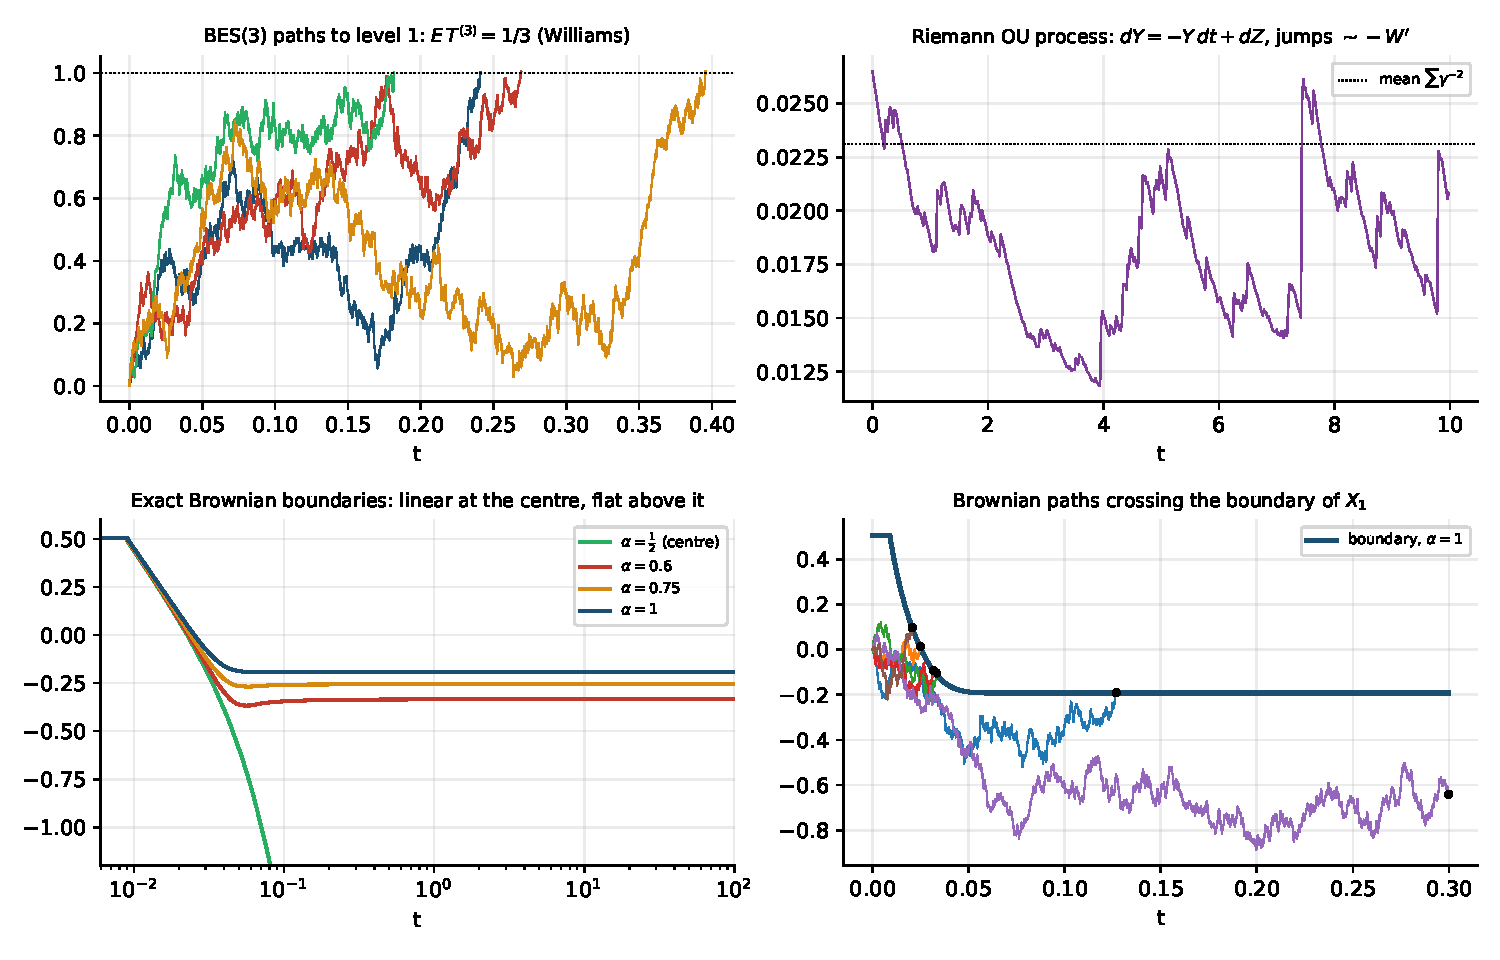
\includegraphics[width=\textwidth]{fig/bp1_paths.pdf}
\caption{Four processes of the map. Top left: paths of a three dimensional Bessel process run until they reach the level one; the hitting time has mean $\frac13$, and two independent copies make up the variable $S_2$ of Section~\ref{bp:sec:mellin}. Top right: ten units of time of the Riemann Ornstein Uhlenbeck process $F$, written $Y$ in the plot, whose stationary law is the centre clock, with the mean $\E T$, written $\sum\gamma^{-2}$ in the plot. Bottom left: the exact Brownian boundaries of $T_\alpha$ at $\alpha=\frac12$, $0.6$, $0.75$ and $1$, those at $0.6$ and $0.75$ computed under RH beyond $t=0.03$ (Section~\ref{bp:sec:across}), asymptotically linear at the centre and flat above it. Bottom right: Brownian paths crossing the boundary of $T_1$, written $X_1$ in the plot (Section~\ref{bp:sec:rs1}). Drawn by \texttt{figs.py} in the folder \texttt{basepoint\_one/process\_map} from the output of \texttt{ou.py}, the boundaries of \texttt{bnd\_alpha.py} at $\alpha=0.6$ and $0.75$, and those of Sections~\ref{ch:boundaries} and \ref{ch:bphit} at the centre and at the basepoint one.}
\label{pm:fig:paths}
\end{figure}

\subsection{Subordinated Brownian motion and the map of processes}\label{pm:sec:map}

Running an independent standard Brownian motion $B$ on a clock gives a symmetric law with
\[
\E e^{iuB_{T_\alpha}}=\E e^{-u^2T_\alpha/2}=\frac{\xi(\alpha)}{\xi(\alpha+|u|/\sqrt2)},\qquad u\in\R,
\]
so $B_{T_\alpha}$ has the law of $Y_\alpha/\sqrt2$, the normal scale mixture of Proposition~\ref{sm:prop:cf}, and what Section~\ref{ch:strip} proves for $Y_\alpha$ carries over with a factor $\sqrt2$. The characteristic function exists at every basepoint with no hypothesis. At the centre $B_T$ has the finite variance $\E T$; above it the characteristic function has a corner at the origin, $B_{T_\alpha}$ lies in the domain of attraction of the Cauchy law, and $P(|B_{T_\alpha}|>y)\sim\sqrt2\,b_\alpha/(\pi y)$ as $y\to\infty$. The law is a symmetric EGGC exactly when $T_\alpha$ is a GGC (Theorems~\ref{sm:thm:thorin} and \ref{sm:thm:strip}), and under RH at the centre it is the sum $\sum_kL_k/(\sqrt2\gamma_k)$ of scaled Laplace variables. Its Cauchy factor, of scale $b_\alpha/\sqrt2$, comes from the constant $b_\alpha/\pi=v_\alpha(0)/\pi$ of the Thorin density wherever the Thorin form \eqref{sm:eq:thorin} holds, and the planar Brownian reading of Section~\ref{bp:sec:planar} holds at every basepoint $\alpha$ to the right of every zero: $v_\alpha(\theta)\,d\theta/\pi=\sum_\rho P(B^2_H\in d\theta\mid B_0=\rho)$, where $B=(B^1,B^2)$ is a planar Brownian motion and $H$ is now its first time to reach the line $\re s=\alpha$. So the constant $b_\alpha/\pi$ is the density at $\theta=0$ of this sum of harmonic measures. Table~\ref{pm:tab:bm}, computed by \texttt{comp2.py}, checks the characteristic function and the tail at three basepoints with $3\times10^5$ draws of $T_\alpha$ each, from the subordination identity, with the tilted clock drawn as for Table~\ref{sm:tab:mc}.

\begin{table}[htbp]
\centering\small
\setlength{\tabcolsep}{4pt}
\begin{tabular}{ccccccc}
\toprule
$\alpha$ & \begin{tabular}[b]{@{}c@{}}$u=1$,\\ Monte Carlo\end{tabular} & exact & \begin{tabular}[b]{@{}c@{}}$u=3$,\\ Monte Carlo\end{tabular} & exact & $y\,P(|B_{T_\alpha}|>y)$, $y=10$ & $\sqrt2\,b_\alpha/\pi$\\
\midrule
0.6 & 0.98546 & 0.98530 & 0.89322 & 0.89286 & 0.0024 & 0.0021\\
0.75 & 0.98050 & 0.98049 & 0.87989 & 0.87994 & 0.0050 & 0.0052\\
1 & 0.97273 & 0.97253 & 0.85933 & 0.85888 & 0.0095 & 0.0104\\
\bottomrule
\end{tabular}
\caption{The characteristic function $\xi(\alpha)/\xi(\alpha+|u|/\sqrt2)$ of subordinated Brownian motion, estimated by the mean of $\cos(uB_{T_\alpha})$ over $3\times10^5$ draws at each basepoint, and its Cauchy type tail; the tail estimates rest on $72$, $149$ and $284$ exceedances of $y=10$. Computed by \texttt{comp2.py} in the folder \texttt{basepoint\_one/process\_map}.}
\label{pm:tab:bm}
\end{table}

Figure~\ref{pm:fig:map} and Table~\ref{pm:tab:map} arrange the processes of Chapter~\ref{chap:basepoint} and of this section by basepoint; we write $a=\alpha-\frac12$. The Mellin side is the Bessel picture of Williams \cite{Williams90} and of Biane, Pitman and Yor \cite{BPY01}: $S_2$, the sum of two independent hitting times of the level one by a three dimensional Bessel process, satisfies $\E(\pi S_2/2)^{s/2}=2\xi(s)$ (Section~\ref{ch:clock}), and $V_\alpha$ is $\frac12\log(\pi S_2/2)$ under the law of $S_2$ size biased by $S_2^{\alpha/2}$ (Section~\ref{bp:sec:mellin}). The clock side starts from the centre clock, which under RH with simple zeros is Kent's hitting time for a string with spectrum $\{\gamma^2\}$, and passes through the tilt $e^{-a^2T}$ and the sticky Brownian subordination of Theorem~\ref{bp:thm:alpha} to $T_\alpha$. From $T_\alpha$ it continues to the Wiener gamma integral of Section~\ref{pm:sec:wg}, to Brownian motion run on the clock, and to the Brownian boundaries of Section~\ref{bp:sec:across}, which are asymptotically linear at the centre and, at the basepoints computed, flat above it, with the Wald defect $\E\,b(T_\alpha)=b_\alpha/\sqrt2$ in place of Wald's identity when the boundary is bounded at infinity.

\begin{figure}[htbp]
\centering
\begin{tikzpicture}[node distance=0.55cm and 0.35cm, every node/.style={font=\footnotesize}, box/.style={draw, rounded corners, align=center, minimum width=3.9cm, minimum height=0.8cm, inner sep=2pt}, arr/.style={-latex, thick}]
\node[box, fill=blue!8] (bes) {two $\mathrm{BES}(3)$ hitting times\\ $S_2$, mean $\frac23$\\ (Williams; Biane, Pitman, Yor)};
\node[box, fill=blue!8, right=1.6cm of bes] (polya) {P\'olya variable $V_{1/2}$ and\\ size biased $V_\alpha$ ($S_2^{\alpha/2}$)};
\node[box, fill=green!10, below=of bes] (clock) {centre clock $T$, infinitely\\ divisible and self decomposable\\ with no hypothesis};
\node[box, fill=green!10, right=1.6cm of clock] (kent) {Kent string, spectrum $\gamma^2$\\ (under RH, simple zeros)};
\node[box, fill=orange!12, below=of clock] (sub) {tilt $e^{-a^2T}$, then sticky Brownian\\ inverse local time $u+2a\sqrt u$};
\node[box, fill=orange!12, right=1.6cm of sub] (xa) {$T_\alpha$: GGC if and only if\\ no zero has $\beta>\alpha$};
\node[box, fill=red!8, below=of sub] (ou) {Ornstein Uhlenbeck process\\ driven by $Z$, jump density $-W'$};
\node[box, fill=red!8, right=1.6cm of ou] (wg) {Wiener gamma integral\\ against the smoothed count};
\node[box, fill=gray!10, below=of ou] (bm) {$B_{T_\alpha}$: characteristic function\\ $\xi(\alpha)/\xi(\alpha+|u|/\sqrt2)$};
\node[box, fill=gray!10, right=1.6cm of bm] (bd) {Brownian boundary: asymptotically\\ linear ($\alpha=\frac12$), flat where\\ computed ($\alpha>\frac12$)};
\draw[arr] (bes) -- node[above,font=\scriptsize]{Mellin} (polya);
\draw[arr] (bes) -- node[left]{$1/\Xi$} (clock);
\draw[arr] (clock) -- (kent);
\draw[arr] (clock) -- (sub);
\draw[arr] (sub) -- (xa);
\draw[arr] (clock.west) to[bend right=35] (ou.west);
\draw[arr] (xa) -- (wg);
\draw[arr] (xa) -- (bm);
\draw[arr] (xa.east) to[bend left=35] (bd.east);
\end{tikzpicture}
\caption{Processes attached to $\xi(\alpha+\cdot)$, with $a=\alpha-\frac12$. By rows from the top: the Mellin side, the centre clock, the basepoint clocks, and two rows of further representations. Drawn in TikZ from Table~\ref{pm:tab:map}.}
\label{pm:fig:map}
\end{figure}

\begin{table}[htbp]
\centering\scriptsize
\setlength{\tabcolsep}{3pt}
\begin{tabular}{p{0.15\textwidth}p{0.18\textwidth}p{0.2\textwidth}p{0.18\textwidth}p{0.17\textwidth}}
\toprule
 & \raggedright $\alpha=\frac12$ & \raggedright $\frac12<\alpha<1$ & \raggedright $\alpha=1$ & $\alpha>1$\tabularnewline
\midrule
\raggedright Mellin side & \raggedright P\'olya variable, $S_2^{1/4}$ bias & \raggedright $S_2^{\alpha/2}$ bias & \raggedright $S_2^{1/2}$ bias & $S_2^{\alpha/2}$ bias\tabularnewline
\raggedright L\'evy form of $\log\xi(\alpha+s)$ & \raggedright none: the characteristic function vanishes at the ordinates & \raggedright exists if $\sup\re\rho<\alpha$, only if $\sup\re\rho\le\alpha$ & \raggedright compensated limit, by the prime number theorem & \raggedright absolutely convergent; quasi infinitely divisible\tabularnewline
\raggedright clock law & \raggedright $T$, infinitely divisible and self decomposable & \raggedright $\widetilde T_\alpha+H_{\sqrt2a\widetilde T_\alpha}$ & \raggedright $\widetilde T+H_{\widetilde T/\sqrt2}$ & $\widetilde T_\alpha+H_{\sqrt2a\widetilde T_\alpha}$\tabularnewline
\raggedright GGC & \raggedright if and only if RH & \raggedright if and only if no zero has $\beta>\alpha$ & \raggedright yes & yes\tabularnewline
\raggedright Thorin measure & \raggedright $\sum_{\gamma>0}\delta_{\gamma^2}$ (RH) & \raggedright Cauchy widths $\alpha-\beta$ & \raggedright Cauchy widths $1-\beta$ & Cauchy widths $\alpha-\beta$\tabularnewline
\raggedright Kent string & \raggedright spectrum $\gamma^2$ (RH) & \raggedright spectrum $\gamma^2+a^2$ on the sticky clock (RH) & \raggedright spectrum $|\rho|^2$ on the sticky clock (RH) & \raggedright spectrum $\gamma^2+a^2$ on the sticky clock (RH)\tabularnewline
\raggedright tail of the clock & \raggedright exponential, rate $\gamma_1^2$ & \raggedright $b_\alpha(\pi x)^{-1/2}$ & \raggedright $0.01303\,x^{-1/2}$ & $b_\alpha(\pi x)^{-1/2}$\tabularnewline
\raggedright Brownian boundary & \raggedright asymptotically linear, slope $-\sqrt2\gamma_1$ & \raggedright flat: $-0.3338$ ($\alpha=0.6$), $-0.2554$ ($\alpha=0.75$) & \raggedright flat at $-0.19277$ & flat\tabularnewline
\raggedright Wald defect $\E\,b(T_\alpha)$ & \raggedright $0$ & \raggedright $b_\alpha/\sqrt2$ & \raggedright $\sum_\rho\rho^{-1}/\sqrt2$ & $b_\alpha/\sqrt2$\tabularnewline
\raggedright $B_{T_\alpha}$ & \raggedright finite variance & \raggedright Cauchy domain & \raggedright Cauchy domain, tail $0.0104/y$ & Cauchy domain\tabularnewline
\raggedright Ornstein Uhlenbeck driver & \raggedright jump density $-W'$ & \raggedright jump density $-W_\alpha'$ & \raggedright jump density $-k_1'$ & jump density $-k_\alpha'$\tabularnewline
\raggedright symmetric EGGC $Y_\alpha$ & \raggedright if and only if RH & \raggedright if and only if no zero has $\beta>\alpha$ & \raggedright yes & yes\tabularnewline
\bottomrule
\end{tabular}
\caption{The processes by basepoint, with $a=\alpha-\frac12$. (RH) marks statements that hold under RH, and the Kent strings need the zeros to be simple as well. The Mellin row gives the size bias of $S_2$ that produces $V_\alpha$ (Section~\ref{bp:sec:mellin}); $\widetilde T_\alpha$, $H$ and the sticky clock are those of Theorem~\ref{bp:thm:alpha} and Corollary~\ref{bp:cor:kent}, with $\widetilde T=\widetilde T_1$; the boundaries $b$ and their Wald defects are those of Sections~\ref{bp:sec:rs1} and \ref{bp:sec:across}; $Y_\alpha=\sqrt2B_{T_\alpha}$ in law (Proposition~\ref{sm:prop:cf}); and $k_\alpha(x)\,dx/x$ is the L\'evy measure of $T_\alpha$. The boundary row reports computations at $\alpha=\frac12$, $0.6$, $0.75$ and $1$, those at $0.6$ and $0.75$ made under RH beyond $t=0.03$, and its entry for $\alpha>1$ is extrapolated, not computed; the flatness is observed, not proved, and above the centre the Wald defect $b_\alpha/\sqrt2$ requires the boundary to be bounded at infinity (Lemma~\ref{bp:lem:wald}). All other entries hold as stated.}
\label{pm:tab:map}
\end{table}

Three conclusions come out of the map. First, the Mellin side and the clock side differ in kind. The Bessel picture and the size biased variables $V_\alpha$ built from it are unconditional at every basepoint, and on that side the zeros enter only as zeros, of the characteristic function $\Xi(t)/\Xi(0)$ of the P\'olya variable and of $\xi(\alpha+s)$ in the L\'evy forms of Section~\ref{sb:sec:qid}; the positivity statements equivalent to RH, the GGC property of the centre clock and the EGGC property of $Y_{1/2}$, live on the clock side, in the reciprocal, and so does the Kent string, which needs simple zeros as well.

Second, on the clock side the Ornstein Uhlenbeck process at the centre and, at every basepoint above it, the tilted and subordinated clock, Brownian motion run on the clock and the Brownian boundary exist with no hypothesis. What changes with $\alpha$ is whether $T_\alpha$ is a GGC, that is, whether it has a positive Thorin measure, which decides whether the Wiener gamma representation and the symmetric EGGC property are available: always for $\alpha\ge1$, for $\frac12<\alpha<1$ exactly when no zero has real part greater than $\alpha$, whatever the sign of $v_\alpha$ on the line (Remark~\ref{rem:ch2:oneline}), and under RH at the centre. The Kent strings need RH at every basepoint, and simple zeros as well, because a Kent hitting time is a GGC whose Thorin measure consists of unit atoms at distinct points (Section~\ref{bp:sec:kent}). Under RH with simple zeros the tilted clock $\widetilde T_\alpha$ is Kent's hitting time for a string with spectrum $\{\gamma^2+a^2\}$, and $T_\alpha$ is the hitting time of the string diffusion run on the local time of a sticky Brownian motion (Corollary~\ref{bp:cor:kent}, at $\alpha=1$). The shifted clock $T_\alpha$ itself is never a Kent hitting time for $\alpha>\frac12$: when it is a GGC, each pair of zeros $\rho,\bar\rho$ with $\beta<\alpha$, such as those on the critical line, contributes to its Thorin measure the pair of Cauchy kernels of width $\alpha-\beta$ at $\pm\gamma$ (Section~\ref{sb:sec:bernstein}), so that measure is not a sum of atoms.

Third, the Bessel process is the template. Its hitting time of the level one is Kent's hitting time for a string with spectrum $\{\pi^2n^2/2\}$, and under RH with simple zeros the centre clock is Kent's hitting time for a string with spectrum $\{\gamma^2\}$. The processes computed here show what such a string would do, and the basepoints inside the strip show how the picture degrades, continuously and quantitatively, as positivity is pushed towards the centre.
